\usetikzlibrary {circuits.logic.US, calc}
\usetikzlibrary{decorations.markings}
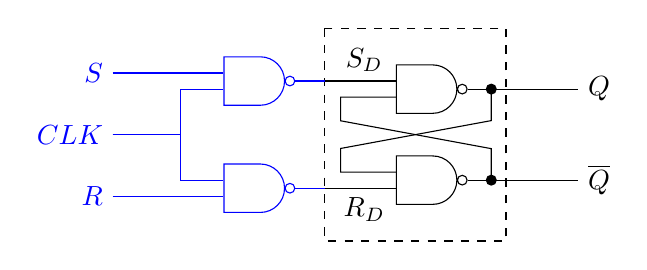
\begin{tikzpicture}[circuit logic US]
  % elements
  \matrix[column sep=30, row sep=15]
  {
    \node [nand gate] (n3) {}; \\
    \node [nand gate] (n4) {}; \\
  };
  \node [blue, nand gate, left, xshift=-40] (n1) at (n3.input 1) {};
  \node [blue, nand gate, left, xshift=-40] (n2) at (n4.input 2) {};

  % labels
  \node[blue, left, xshift=-40] (s)   at (n1.input 1) {$S$};
  \node[blue, left, xshift=-40] (r)   at (n2.input 2) {$R$};
  \node[blue, left, xshift=-40] (clk) at ($(n1.input 1)!0.5!(n2.input 2)$) {$CLK$};
  \node[right, xshift=40] (q)   at (n3.output) {$Q$};
  \node[right, xshift=40] (nq)  at (n4.output) {$\overline{Q}$};

  \node[above] (sd) at ($(n3.input 1) + (left:0.4)$) {$S_D$};
  \node[below] (rd) at ($(n4.input 2) + (left:0.4)$) {$R_D$};

  % lines
  \draw[blue] (s) -- (n1.input 1);
  \draw[blue] (r) -- (n2.input 2);
  \draw[blue] (clk) -- ++(right:1.4) |- (n1.input 2);
  \draw[blue] (clk) -- ++(right:1.4) |- (n2.input 1);
  % \draw (n1.output) |- (n3.input 1);
  % \draw (n2.output) |- (n4.input 2);
  \draw (n3.output) -- (q);
  \draw (n4.output) -- (nq);
  \draw[postaction={decorate,decoration={markings,mark=at position 1 with {\fill circle (2pt);}}}]
    (n3.input 2) -- ++(left:0.7) -- ++(down:0.3)
                 -- ($(n4.output)+(right:0.3)+(up:0.4)$)
                 -- ($(n4.output)+(right:0.3)$);
  \draw[postaction={decorate,decoration={markings,mark=at position 1 with {\fill circle (2pt);}}}]
    (n4.input 1) -- ++(left:0.7) -- ++(up:0.3)
                 -- ($(n3.output)+(right:0.3)+(down:0.4)$)
                 -- ($(n3.output)+(right:0.3)$);

  \coordinate (ls) at ($(sd)+(-0.5,0)$);
  \coordinate (lr) at ($(rd)+(-0.5,0)$);
  \draw[dashed] ($(sd)+(-0.5, 0.4)$) rectangle ($(rd)+(1.8, -0.4)$);
  \draw[blue] (n1.output) -- (ls |- n1.output);
  \draw (ls |- n1.output) --(n3.input 1);
  \draw[blue] (n2.output) -- (lr |- n2.output);
  \draw (lr |- n2.output) --(n4.input 2);

\end{tikzpicture}